\documentclass[a4paper,14pt]{article} % тип документа
%\documentclass[14pt]{extreport}
\usepackage{extsizes} % Возможность сделать 14-й шрифт


\usepackage{geometry} % Простой способ задавать поля
\geometry{top=25mm}
\geometry{bottom=35mm}
\geometry{left=20mm}
\geometry{right=20mm}
%%%Библиотеки
	%\usepackage[warn]{mathtext}	
	\usepackage[T2A]{fontenc} % кодировка
	\usepackage[utf8]{inputenc} % кодировка исходного текста
	\usepackage[english,russian]{babel} % локализация и переносы
	\usepackage{caption}
	\usepackage{listings}
	\usepackage{amsmath,amsfonts,amssymb,amsthm,mathtools}
	\usepackage{wasysym}
	\usepackage{graphicx}%Вставка картинок правильная
	\usepackage{float}%"Плавающие" картинки
	\usepackage{wrapfig}%Обтекание фигур (таблиц, картинок и прочего)
	\usepackage{fancyhdr} %загрузим пакет
	\usepackage{lscape}
	\usepackage{xcolor}
	\usepackage[normalem]{ulem}
	\usepackage{hyperref}

%%%Конец библиотек




%%%Настройка ссылок
	\hypersetup
	{
		colorlinks=true,
		linkcolor=blue,
		filecolor=magenta,
		urlcolor=blue
	}
%%%Конец настройки ссылок


%%%Настройка колонтитулы
	\pagestyle{fancy}
	\fancyhead{}
	\fancyhead[L]{Вопрос по выбору}
	\fancyhead[R]{Талашкевич Даниил, группа Б01-009}
	\fancyfoot[C]{\thepage}
%%%конец настройки колонтитулы



							\begin{document}
						%%%%Начало документа%%%%


%%%Начало титульника
\begin{titlepage}

	\newpage
	\begin{center}
		\normalsize Московский физико-технический институт \\(госудраственный 			университет)
	\end{center}

	\vspace{6em}

	\begin{center}
		\Large Устный экзамен по физике \\(электричество и магнетизм) \\
        \Large Вопрос по выбору
	\end{center}

	\vspace{1em}

	\begin{center}
		\Large \textbf{Доменная структура ферромагнетиков}
	\end{center}

	\vspace{2em}

	\begin{center}
		\large Талашкевич Даниил Александрович\\
		Группа Б01-009
	\end{center}

	\vspace{\fill}

	\begin{center}
	Долгопрудный \\2021
	\end{center}
	
\end{titlepage}
%%%Конец Титульника



%%%Настройка оглавления и нумерации страниц
	\thispagestyle{empty}
	\newpage
	\tableofcontents
	\newpage
	\setcounter{page}{1}
%%%Настройка оглавления и нумерации страниц


					%%%%%%Начало работы с текстом%%%%%%
				
\section{Ферромагнетизм}

Ферромагнетиками называют твердые тела, которые могут обладать спонтанной намагниченностью, т.е. намагничены уже в отсутствии магнитного поля. Типичными представителями ферромагнетиков являются металлы: железо, кобальт, никель. Ферромагнетики способны сильно намагничиваться даже в небольших полях.

Характерной особенностью ферромагнетиков является сложная нелинейная зависимость между $\overrightarrow{I}$ и $\overrightarrow{H}$. По мере возрастания $\overrightarrow{H}$ намагниченность $\overrightarrow{I}$ сначала быстро растет, а затем становится практически постоянной: $\overrightarrow{I} = \overrightarrow{I_S}$ (насыщение), т.е. кривая $I = I(H)$ переходит в горизонтальную прямую. Магнитная индукция $\overrightarrow{B} = \overrightarrow{H} + 4\pi\overrightarrow{I}$ также растет с возрастанием поля $\overrightarrow{H}$, а в состоянии насыщения $\overrightarrow{B} = \overrightarrow{H} + 4\pi\overrightarrow{I_S}$.

Ввиду нелинейной связи между $\overrightarrow{I} = \chi\overrightarrow{H}$ и $\overrightarrow{H}$ для ферромагнетиков магнитная восприимчивость $\chi$ и магнитная проницаемость $\mu = 1 + 4\pi\chi$ могут иметь тензорнный характер(вектора $\overrightarrow{I}$ и $\overrightarrow{H}$ не сонаправлены). Эти функции рассматриваются как функции напряженности поля $\overrightarrow{H}$.

\begin{figure}[H]
	\center{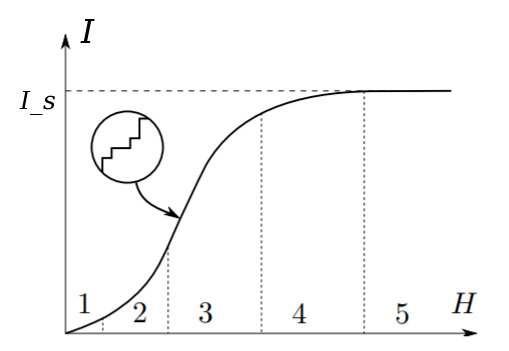
\includegraphics[scale = 0.5]{pic_1.png}}
	\caption{Начальная кривая намагничивания ферромагнетика}
\end{figure}

Вторая характерная особенность ферромагнетиков состоит в том, что для них зависимость $\overrightarrow{I}$ от $\overrightarrow{H}$ не однозначна, а определяется предшествующей историей намагничивания ферромагнитного образца. Это явление называется \textbf{магнитным гистерезисом}. Благодаря гистерезису намагничивание и перемагничивание ферромагнетиков сопровождается выделением тепла, называемого теплом гистерезиса.

\begin{figure}[H]
	\center{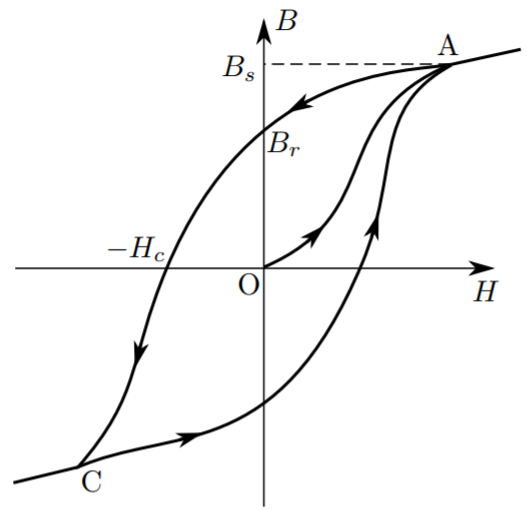
\includegraphics[scale = 0.5]{pic_2.png}}
	\caption{Начальная кривая намагничивания (OA) и предельная петля гистерезиса}
\end{figure}

Третья характерная особенность ферромагнетиков, состоит в том, что для любого ферромагнетика существует определенная температура $T = T_K$ называемая температурой или точкой Кюри, при переходе через которую вещество ферромагнетика претерпевает фазовый переход второго рода. Вещество является ферромагнетиком только при $T < T_K$. При $T > T_K$ вещество становиться парамагнетиком. Магнитная восприимчивость подчиняется закону Кюри-Вейсса 
\[\chi = \frac{Const}{T - T_K}\]

\section{Теория ферромагнетизма Вейсса}

В теории Вейсса силы взаимодействия между атомами формально сводятся к "эффективному" полю, которое и ориентирует атомы ферромагнетика. Эффективное поле складывается из обычного макроскопического поля в веществе $\overrightarrow{H}$ и некоторого гипотетического "молекулярного поля". Согласно предположению Вейсса:

\[\overrightarrow{B_\text{эфф}} = \overrightarrow{H} + b\overrightarrow{I}\]

где $b$ -- некоторая положительная постоянная, характеризующая свойства различных ферромагнетиков. Она называется постоянной Вейсса.

Исходя из этих предположений, рассчитаем намагничивание ферромагнетика $I$. Для этого заменим в теории Ланжевена поле $\overrightarrow{H}$ на эффективное поле $B_\text{эфф}$.

\[I = n\mathfrak{M}L(x)\]

\[x = \frac{\mathfrak{M}B_\text{эфф}}{kT} = \frac{\mathfrak{M}(H + bI)}{kT}\]

Заметим, что $I_S = n\mathfrak{M}$, тогда выразим $I$ из двух предыдущих уравнений:
\[I = I_S L(x), ~I = \frac{kTn}{I_S b}x - \frac{H}{b}\]

Исследуем эту систему графически. Будем откладывать по горизонтальной оси величину x, а по вертикальной -- намагничивание I.

\begin{figure}[H]
	\center{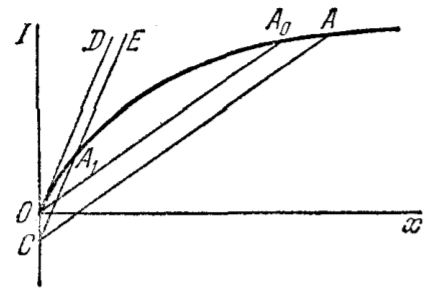
\includegraphics[scale = 0.6]{pic_3.png}}
	\caption{График I(x)}
\end{figure}

Допустим сначала, что наклон прямой CA меньше наклона кривой
\[\frac{kTn}{I_Sb} < I_S\left(\frac{dL}{dx}\right)_{x=0}\]
\[T < \frac{I_S^2 b}{kn}\left(\frac{dL}{dx}\right)_{x=0} = T_K\]
Прямая пересечет прямую Ланжевена в точке A, оридината и будет намагничиванием ферромагнетика I.

Если уменьшать поле H до нуля точка C будет подниматься к точке O, а точка A -- перемещаться к точке $A_0$. Когда поле H обратиться в нуль, ферромагнетик останется намагниченным -- его намагничивание представится ординатой точки $A_0$. 

Стоит отметить, что ферромагнетик будет спонтанно намагничен и в том случае, когда он вообще не вносился ни в какое магнитное поле, потому что благодаря гипотетическому взаимодействию между атомами, введенному Вейсом, состояние спонтанного намагничивания "энергетически выгодно".

Таким образом, при $T < T_K$ ферромагнетик должен быть спонтанно намагничен. Энергии теплового движения недостаточно, чтобы разрушить это намагничивание. Величина $T_K$ называется температурой или точкой Кюри.

Ниже точки Кюри из-за наличия спонтанного намагничивания $\chi$ и $\mu$ являются функциями от H:
\[\chi = \frac{dI}{dH},~ \mu = \frac{dB}{dH}\]

Теперь предположим, что наклон прямой CA больше наклона кривой Ланжевена в точке O. Это означает, что $T > T_K$. Тогда при отсутствии магнитного поля прямая CA займет положение OD, т.е. пересечет функцию Лагжевена только в начале координат. При этом спонтанное намагничивание не возникнет: намагничивание разрушается тепловым движением. Поэтому, чтобы намагнитить необходимо приложить магнитное поле. Прямая CA займет положение CE и пересечет кривую Ланжевена в точке $A_1$. Из эксперементов известно, что ордината $OC = -\frac{H}{b}$ мала, а поэтому мал и учаток $OA_1$ кривой Ланжевена.

\[L(x) = \left(\frac{dL}{dx}\right)_{x=0}x\]

\[I = I_S L(x) = I_S \left(\frac{dL}{dx}\right)_{x=0}x\]

\[T_K = \frac{I_S^2 b}{kn}\left(\frac{dL}{dx}\right)_{x=0} \Rightarrow \left(\frac{dL}{dx}\right)_{x=0} = \frac{T_K k n}{I_S^2b}\]

\[I = \frac{T_K k n}{I_Sb} x = \frac{T_K k n}{I_Sb} \frac{T}{T}x = \frac{T_K}{T}\left(I + \frac{H}{b}\right)\]

\[I = \chi H \Rightarrow \chi = \frac{T_K}{T}\left(\chi + \frac{1}{b}\right) \Rightarrow \chi\left(\frac{T}{T_K} - 1\right) = \frac{1}{b}\]

\[\chi = \frac{T_K}{b(T - T_K)} = \frac{const}{T-T_K}\]

Намагничивание пропорционально полю, т.е. выше точки Кюри ферромагнетик превращается в парамагнетик, причем зависимость магнитной восприимчивости от температуры определяется законом Кюри-Вейсса.

%=====================================================================================

\section{Доменная структура ферромагнетиков}

Как и в случае парамагнетиков, атомы ферромагнетика обладают собственным магнитным моментом. Однако даже в отсутствие внешнего магнитного поля атомы ферромагнетика способны образовывать упорядоченные структуры (домены), в которых все магнитные моменты ориентированы практически в одном направлении. Таким образом, каждый отдельный атом испытывает влияние не только внешнего поля, но и поля, созданного коллективом его соседей.

\subsection{Вступление}

$\textbf{Домены}$ -- макроскопическая область, в которой ориентация вектора намагниченности определенным -- строго упорядоченным -- образом повернута или сдвинута.

Под доменной областью будем понимать область, которая имеет только одно направление намагниченности.

Если весь образец намагничен в одну сторону, то возникает сильное магнитное поле, несущее большую энергию. Но это состояние невыгодно: выгодно разбить образед на намагниченные участки ($\textbf{домены}$). При этом намагниченность разных доменов направлена так, чтобы минимизировать полную магнитную энергию. Рассмотрим доменную структуру: в простейшем случае доменную структуру тонкого образца можно представить, как на рис. $\ref{935}$. Домены с противоположной намагниченностью чередуются. Кроме того, могут появляться так называемые \
$\textbf{замыкающие}$ $\textbf{домены}$ -- треугольные домены сверху и снизу образца (рис. $\ref{935}$), передающие магнитный поток от одного домена к другому и уменьшающие магнитное поле вне вещества.

\begin{figure}[h!]

\begin{center}
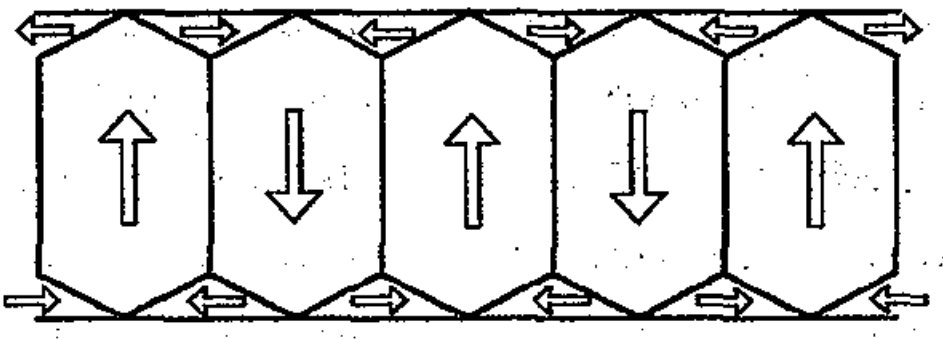
\includegraphics[width=0.3\textwidth]{9.3.5.png} 
\end{center}
\caption{Чередование доменов с противоположной намагниченностью (стрелки указывают направление намагниченности домена)}
\label{935}

\end{figure}

\subsection{Доменная теория}

Для в какой-то степени качественной оценки и для получения объяснений причин непроизвольности размера доменов, а также факторов формирования его, проведем следующие рассуждения:

Рассмотрим плоскую квадратную ферромагнитную пластинку толщиной $h$ с площадью $L^{2} .$

Равновесное распределение вектора намагниченности соответствует минимуму полной энергии пластинки. Полная энергия включает в себя энергию обменного взаимодействия $W_{e}$, энергию магнитной анизотропии $W_{a}$, энергию доменных границ $W_{d}$, энергию $W_{m}$, связанную с возникновением вокруг пластины магнитного поля.

В случае, когда пластинка однородно намагничена, и вектор намагниченности лежит на кристаллографической оси, соответствующей минимуму магнитной анизотропии, достигается минимум суммы $W_{e}+W_{a} .$ С другой стороны, в таком случае очень большой оказывается энергия $W_{m}$, так как вокруг пластины образуется магнитное поле, силовые линии которого далеко выходят из этой пластины. Величина этой энергии будет меньше в том случае, когда меньше магнитное поле вокруг пластины. Такая ситуация реализуется, когда пластина разбивается на области (домены), в каждой из которых вектор намагниченности везде направлен по оси легкого намагничивания, но в соседних доменах направления вектора намагниченности различны. С одной стороны, при такой конфигурации энергия $W_{m}$ уменьшается, но, с другой стороны, с увеличением числа доменов возрастает энергия доменных границ $W_{d}$, так как сосуществование антипараллельных спинов невыгодно с точки зрения энергии обменного взаимодействия.

Энергия $W_{m}$ по величине может быть оценена следующим образом:

\[W_{m}=M^{2} d L^{2},\]

где $d$ -- толщина домена, $M$ -- модуль вектора намагниченности внутри домена.
Энергия доменных границ определяется с помощью поверхностной энергии доменных границ $\sigma:$

\[W_{d}=\sigma L h N,\]

где $N=L / d$ -- число доменных границ. Тогда полная энергия выглядит следующим образом:

\[W_{d}+W_{m}=\sigma L^{2} \frac{h}{d}+M^{2} d L^{2} .\]

Оптимальный размер домена, при котором достигается минимум суммы $W_{d}+W_{m}$, зависит от параметров пластины следующим образом :

\[d_{\text {орt }}^{2}=l_{0} h,\]

где $l_{0}=\frac{\sigma}{M^{2}}$ -- характеристическая длина.

Исходи из этих рассуждений сделаем вывод, что размер домена не может быть произвольным, поскольку в его формировании участвуют несколько конкурирующих факторов:
\begin{enumerate}
    \item необходим выигрыш в энергии за счёт формирования намагниченности в домене благодаря обменному взаимодействию ($\textbf{ориентационная энергия}$).
    \item проигрыш в энергии за счёт возникновения сильных магнитных полей вокруг пластинки (ферромагнетика произвольной формы в общем случае).
    \item проигрыш в энергии за счёт формирования доменных стенок границ соседних доменов с противоположно направленными намагниченностями. В этих стенках происходит переход от одной ориентации намагниченности к другой. В результате теряется выигрыш в ориентационной энергии, что приводит к увеличению поверхностной энергии системы.
\end{enumerate}

\subsection{Перемагничивание ферромагнетика}

Процесс перемагничивания для случая доменной структуры на рис. $\ref{935}$ состоит в том, что доменные стенки начинают смещаться, приводя к $\textbf{поглоще-}$ $\textbf{ию}$ доменов с "неправильной"\ намагниченностью и $\textbf{росту}$ доменов с "правильной"\ намагниченностью, как показано на рис. $\ref{936}$ . Разумеется, движение стенок не сопровождается макроскопическими движениями вещества -- этот процесс состоит только в изменении направления магнитных моментов атомов.

В общем случае ферромагнетик представляет собой набор хаотически ориентированных доменов, в каждом из которых намагниченность имеет определённое направление (рис. $\ref{937}$).

\begin{figure}[h!]

\begin{center}
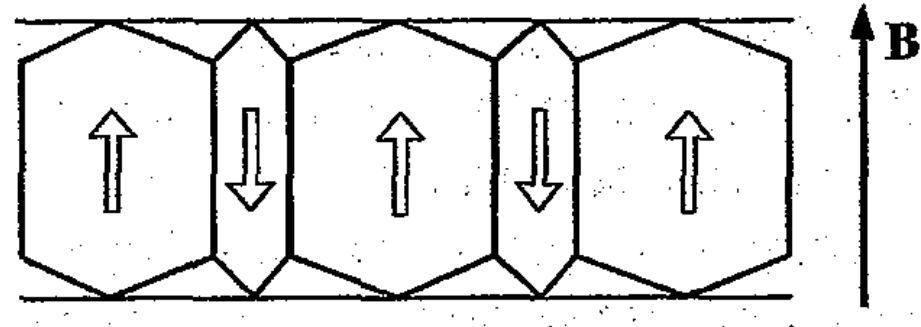
\includegraphics[width=0.3\textwidth]{9.3.6.png} 
\end{center}
\caption{Перемагничивание ферромагнетика путём движения доменных стенок}
\label{936}
\end{figure}

\begin{figure}[h!]

\begin{center}
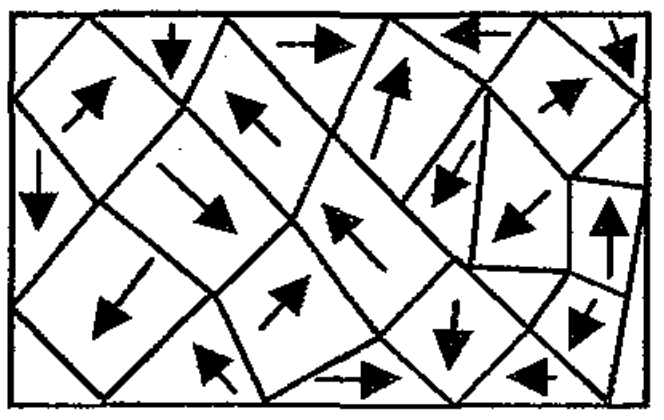
\includegraphics[width=0.3\textwidth]{9.3.7.png} 
\end{center}
\caption{Доменная структура ферромагнетика -- множество  доменов со случайным направлением намагниченности}
\label{937}
\end{figure}

Гистерезисный характер перемагничивания связан с наличием необратимых стадий. Дело в том, что при не слишком высоких полях перемагничивание происходит путём смещения доменной стенки. Но это -- обратимая стадия. Вместе с тем вследствие наличия дефектов структуры движение доменных стенок может происходить неравномерно, скачкообразно. Такие скачки сопровождаются потерями энергии и приводят к тому, что процесс намагничивания становится необратимым, т.е. к гистерезисным явлениям при перемагничивании.

Другой механизм появления необратимости состоит в следующем: в кристаллах существует $\textbf{ось лёгкого намагничивания}$, вдоль которой ориентируется намагниченность. Однако эта ось может не совпадать с направлением внешнего магнитного поля. Такая ситуация обязательно встречается в $\textbf{поликристаллических образцах}$ со случайными ориентациями осей в отдельных кристаллах. И тогда в случае достаточно сильных внешних полей начинается "доворот"\ магнитного момента всего домена к направлению внешнего поля. Эта стадия сопровождается затратами энергии и приводит к гистерезису.

Возможны и другие механизмы, вызывающие потери энергии и гистерезис при перемагничивании. Таковыми являются процессы, когда доменные стенки при своём движении "застревают"\ на дефектах структуры. В результате возникают скачкообразные движения стенок, сопровождающиеся возникновением индукционных токов и соответствующими потерями энергии.

\subsection{Образование доменов}

Остановимся кратко на причине, по которой соседним магнитным моментам выгодно объединяться в домены. В первую очередь подчеркнём, что $\textbf{магнитное}$ (диполь-дипольное) взаимодействие между атомами $\textbf{не может}$ привести к упорядочению системы. Чтобы в этом убедиться, достаточно оценить энергию такого взаимодействия: из квантовой механики известно, что магнитный момент атома по порядку величины равен $\mathfrak{m}_{\mathrm{E}}=9,3 \cdot 10^{-24}$ Дж/Тл (магнетон Бора), характерное расстояние между атомами $a \sim 2 \cdot 10^{-10}$ м, тогда характерное межатомное магнитное поле $B \sim \mu_{0} \frac{\mathfrak{m}_{\mathrm{B}}}{a^{3}} \sim 1$ Тл, и характерная энергия диполь-дипольного взаимодействия $U_{\text {дип. }} \sim \mathfrak{m}_{\mathrm{B}} B \sim 10^{-4}{ }_{\ni \mathrm{B}}$. При такой энергии связи тепловое движение обеспечит полное разупорядочение уже при $T \sim 1 \mathrm{~K}$.

Единственное взаимодействие, которое способно выстроить в ряд магнитные моменты электронов в атомах при температурах порядка комнатной, -- это $\textbf{электростатическое взаимодействие}$ (его энергия на несколько порядков больше магнитной: $e^{2} /\left(4 \pi \varepsilon_{0} a\right) \sim 1$ эВ). Как следует из квантовой механики, если магнитные моменты (или спины) электронов соседних атомов сонаправлены, их электростатическое отталкивание становится меньше. Таким образом, магнитным моментам атомов энергетически выгодно ориентироваться в одном направлении. Такое явление получило название $\textbf{обменного}$ $\textbf{взаимодействия}$.

С другой стороны, магнитное (диполь-дипольное) взаимодействие между доменами препятствует выстраиванию всех магнитных моментов среды в одном направлении. Действительно, энергия такого взаимодействия будет минимальной при  $\textbf{антипараллельном}$ расположении магнитных моментов соседних элементов среды. Поэтому при определённом поперечном размере домена оказывается энергетически выгодно иметь соседний домен с противоположно ориентированным моментом (см. рис. $\ref{42}$ слева).

Наложение внешнего поля заставляет домены ориентироваться по нему, что приводит к резкому увеличению намагниченности образца, а при достаточно большом поле достигается состояние $\textbf{насыщения}$, когда все домены ориентируются по полю (см. рис. $\ref{42}$ справа).

\begin{figure}[h!]

\begin{center}
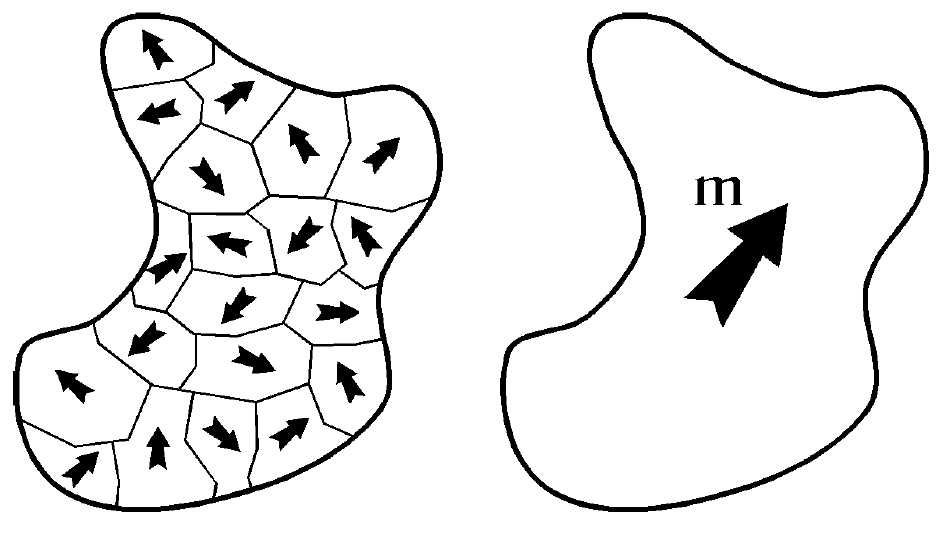
\includegraphics[width=0.4\textwidth]{4.2.png} 
\end{center}
\caption{Доменная структура ферромагнетика при слабом ($\textbf{слева}$) и сильном ($\textbf{справа}$) внешнем поле}
\label{42}
\end{figure}


\section{Литература}

\begin{enumerate}

\item \textbf{Лабораторный практикум по общей физике:} Учебное пособие. В трех томах. Т. 2. Электричество и магнетизм /Гладун А.Д., Александров Д.А., Берулёва Н.С. и др.; Под ред. А.Д. Гладуна - М.: МФТИ, 2007. - 280 с.

\item \text{http://www.amtc.ru/production/metall/Gadoliniy}

\end{enumerate}		
		


\end{document}